

 \cite{Gelman96posteriorpredictive} in a posterior checking framework, but unfortunately we were not able to explore other bayesian criticism measures \cite{Box1980}, because of the difficulty of sampling from this highly peaked and multimodal posterior distribution. 
\\Before comenting results, in figure 2 are shown all the stages of the algorithm in a sample dataset.
\pagebreak 
   \begin{figure}[ht!]
        \centering
        \begin{subfigure}[b]{0.5\textwidth}
                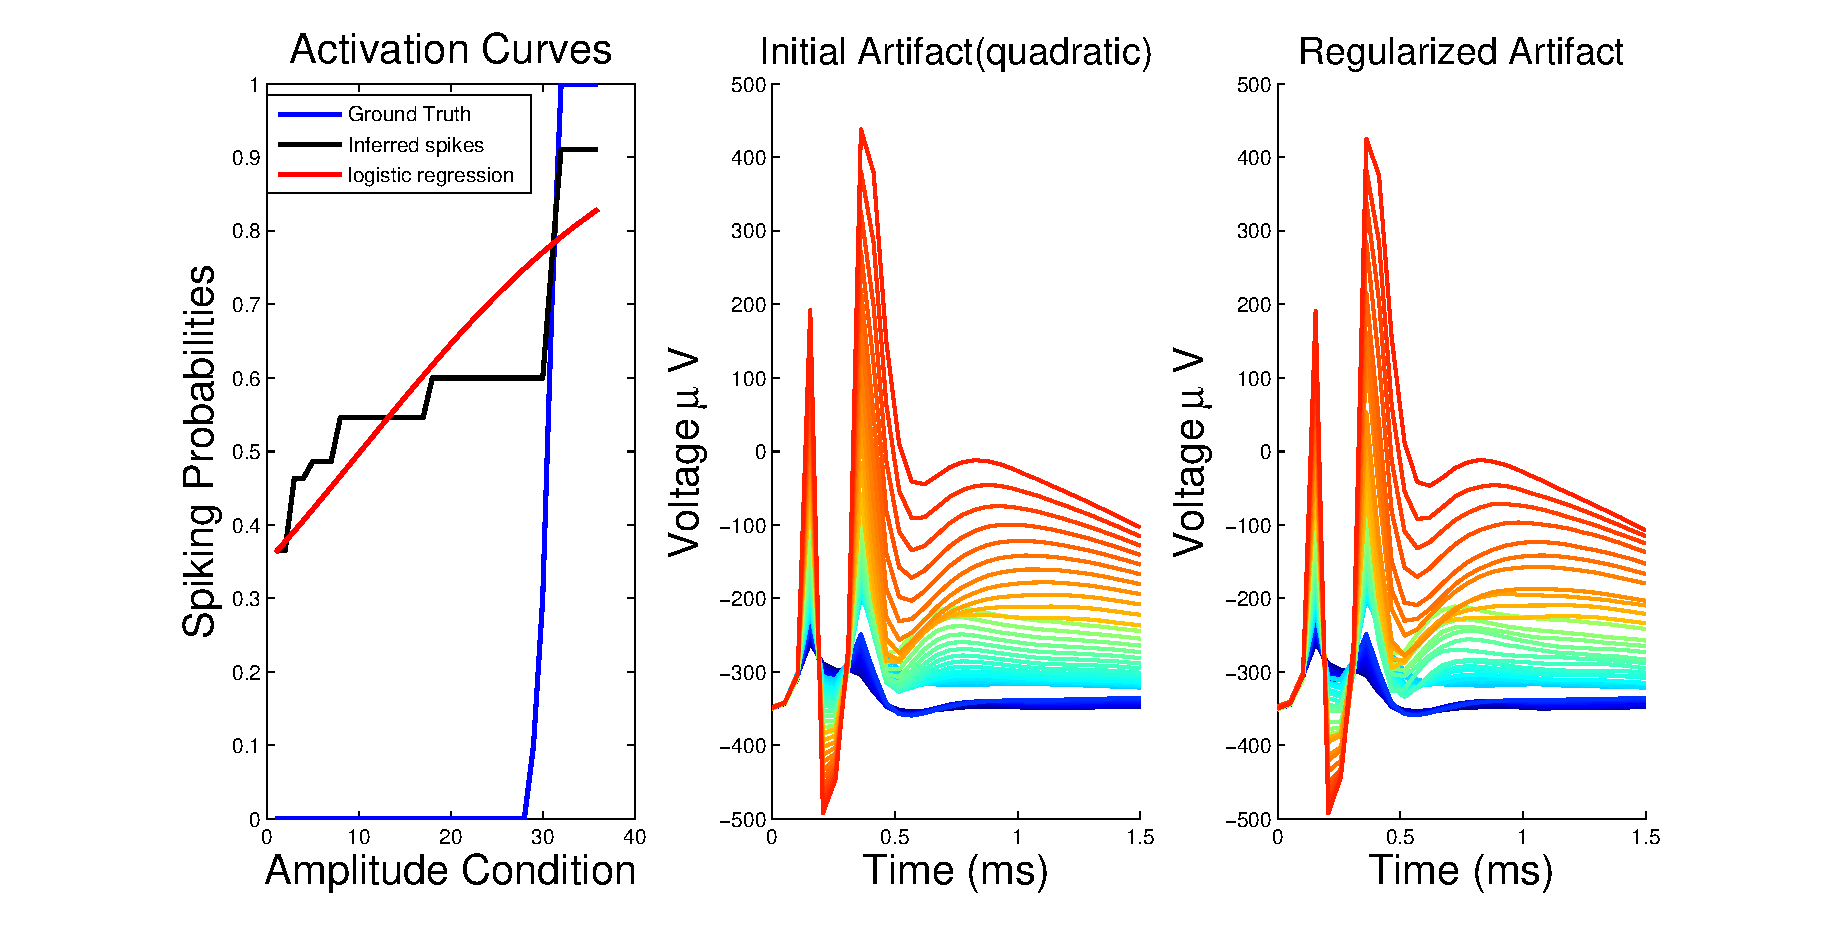
\includegraphics[width=\textwidth]{i0.eps}
                \caption{After Convex relaxation}
                \label{fig:gull}
        \end{subfigure}% 
~\begin{subfigure}[b]{0.5\textwidth}
                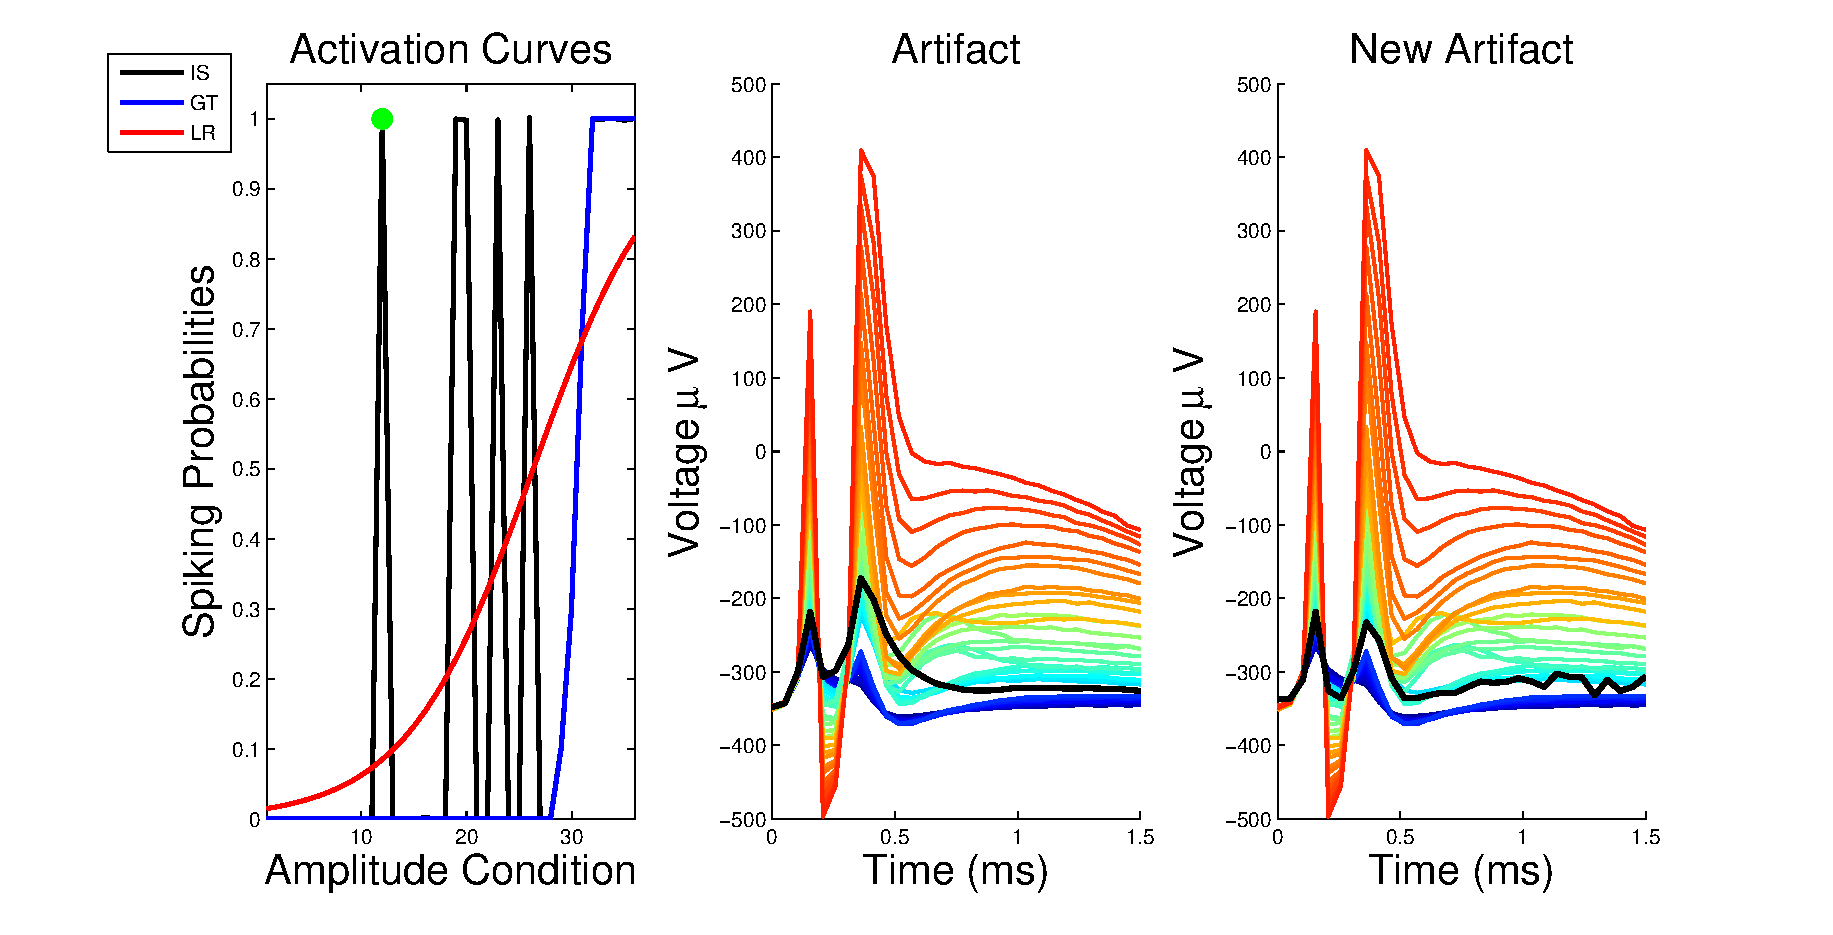
\includegraphics[width=\textwidth]{i1.eps}
                \caption{Gibbs Sampler Solution}
                \label{fig:tiger}
        \end{subfigure}
 
        \begin{subfigure}[b]{0.5\textwidth}
                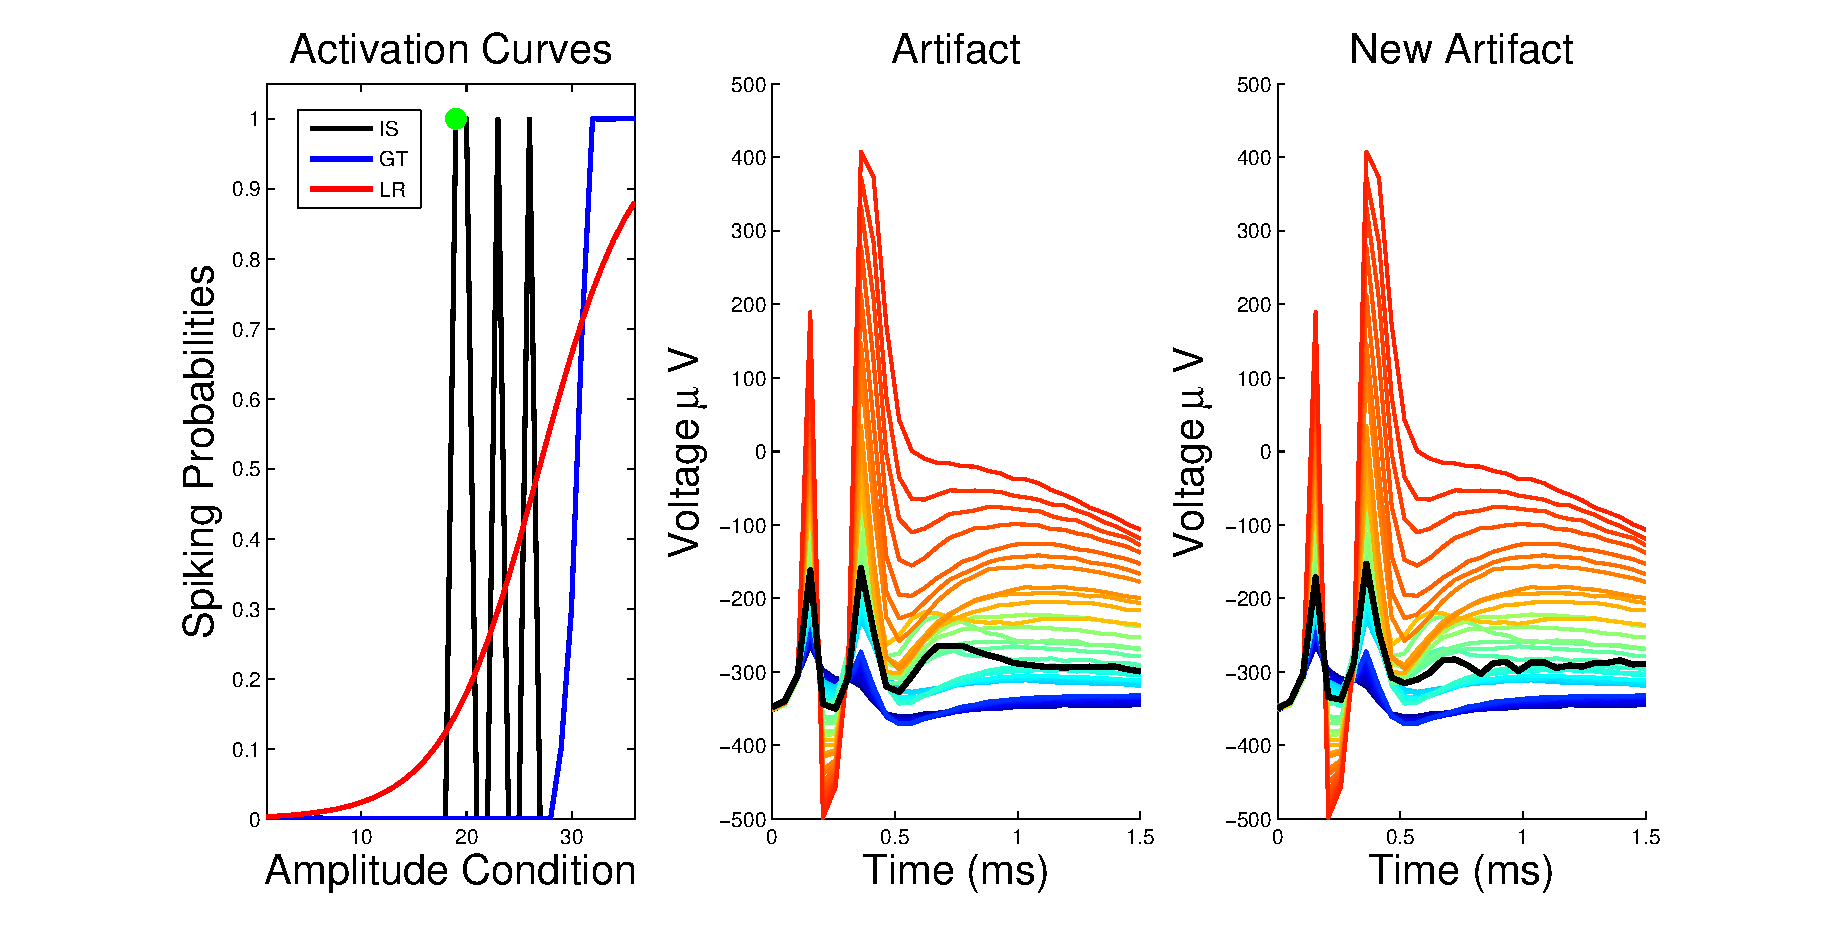
\includegraphics[width=\textwidth]{i2.eps}
                \caption{After one iteration of heuristic}
        \end{subfigure}~
         \begin{subfigure}[b]{0.5\textwidth}
                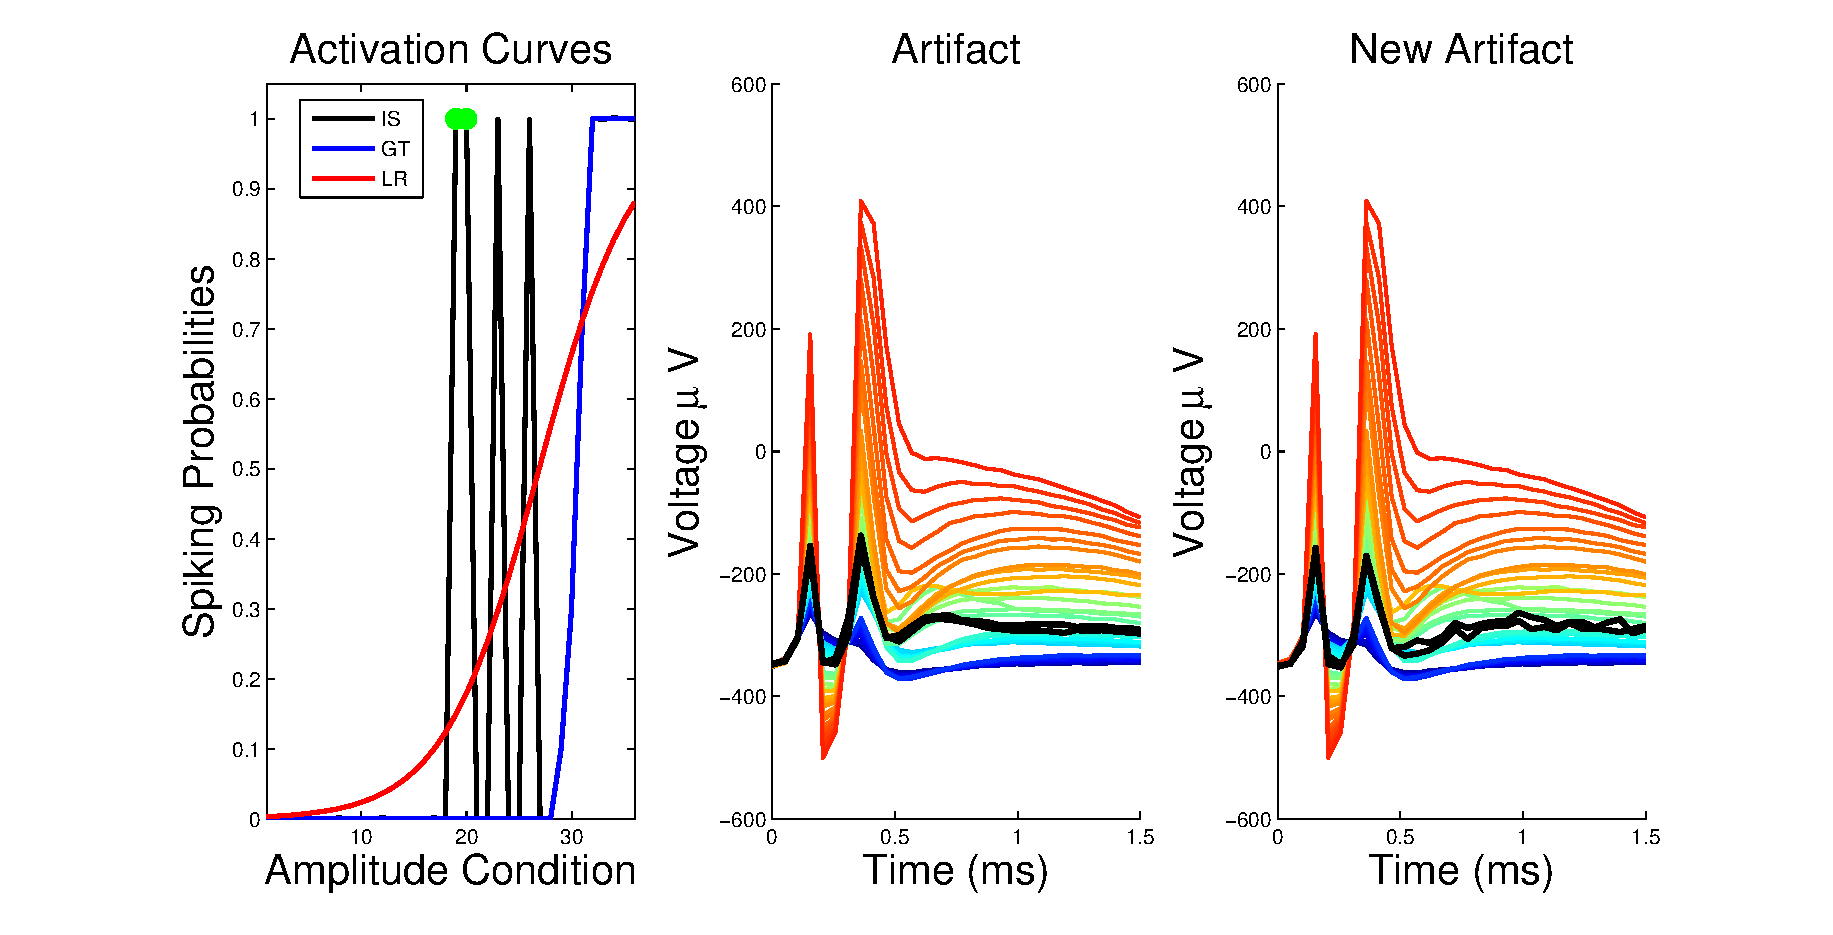
\includegraphics[width=\textwidth]{i3.eps}
                \caption{After two Iterations of heuristic}
                \label{fig:mouse}
        \end{subfigure}
        
        
        \begin{subfigure}[b]{0.5\textwidth}
                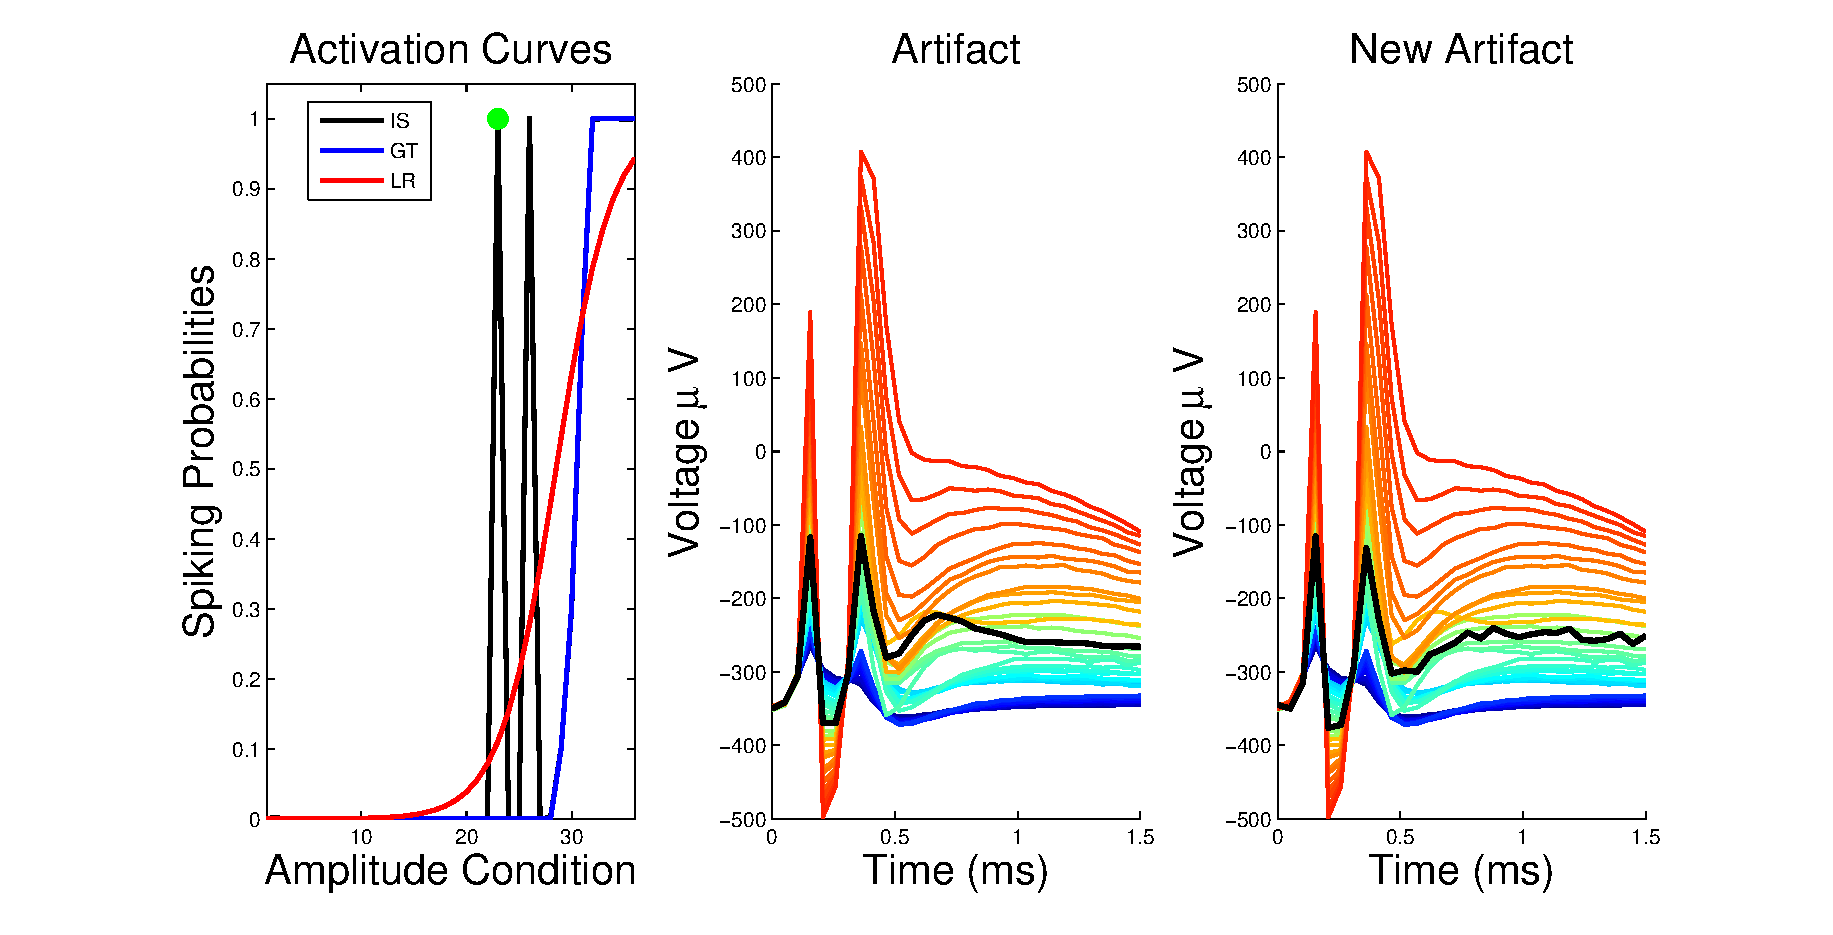
\includegraphics[width=\textwidth]{i4.eps}
                \caption{After three Iterations of heuristic}
        \end{subfigure}~
         \begin{subfigure}[b]{0.5\textwidth}
                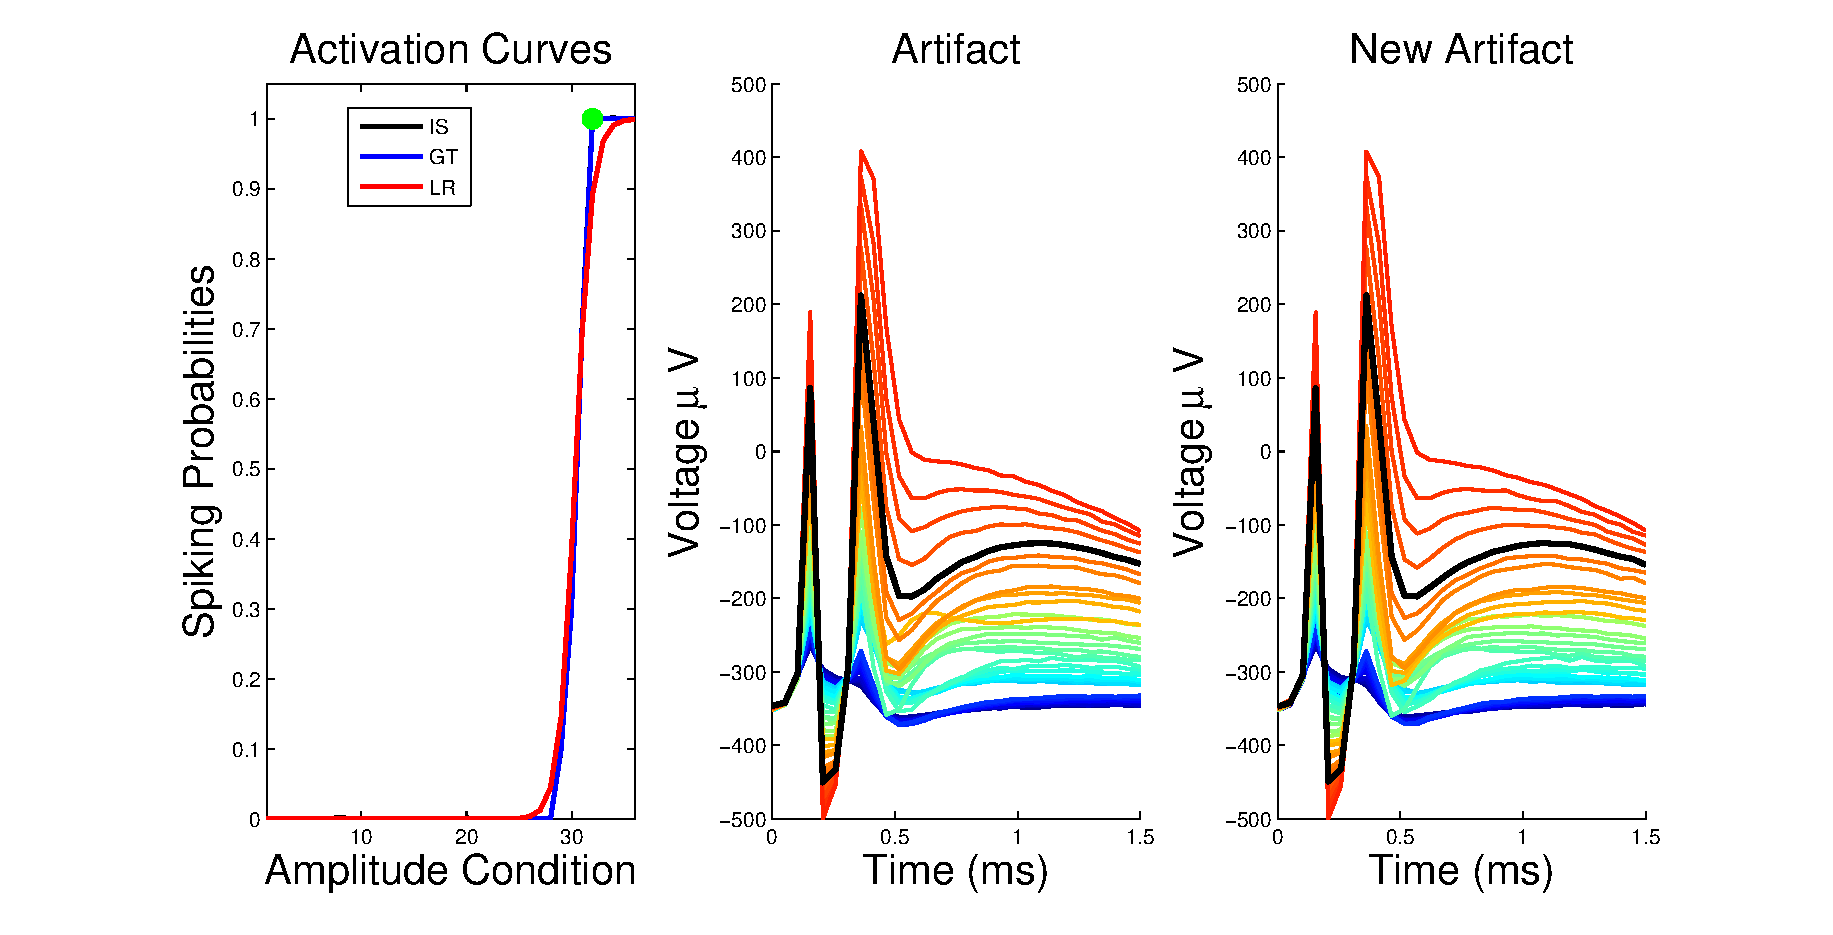
\includegraphics[width=\textwidth]{i6.eps}
                \caption{Final Result}
                \label{fig:mouse}
        \end{subfigure}
\caption{Illustration of the different stages of the algorithm. Initial values provided by the convex relaxation (a) are used as input for the Gibbs sampler (b). If the fit of the activation curve to a logistic model is poor, the artifact is resampled in the conditions that are most responsible of that lack of fit (c,d,e), until no changes are further needed (f)}
\end{figure}


    \section{Results}
    The algorithm was tested in 56 datasets in which spike sorting was required for 4 neurons (templates in the electrodes used are shown in figure 1). For all of them the number of amplitude conditions was 17, and for each condition there were either 20 or 10 trials. In the former performance was almost perfect, with an overall error rate of 0.71\% (see table 1 for summary results for each neuron and figure 3 for the true and estimated activation curves). However, in the latter the error rate was higher, reaching 10.9\% (see table 2 for details), possibly due to the limitations posited by the fewer number of trials. As we aim to decrease the error rate to zero, it is important to understand better which are the causes of failures: Better models can be built if these causes are well understood, and even with the current model this understanding could be used to inform the human expert when the causes are present. It turns out that the unwanted activation of an axonal bundle is the phenomenon that explains the best failures in spike sorting. In the following we show how this axonal activation hampers spike sorting, and how to deal with it in the absence of a better model
    \begin{table}[h!]
\begin{tabular}{|c|c|c|c|c|c|}
\hline
   &  Trials w. spikes & Failures in detection & Trials w. no spikes & False positives  & Total \\ \hline
   Neuron 1 & 1040 & 43 ( 4.1 \%)& 2190 & 73 (3.3\%) & 3230 \\ \hline
   Neuron 2 & 329 & 0 & 2901 & 1 (0.03\%)  & 3230 \\ \hline
   Neuron 3 & 546 & 0 & 2684 & 0 & 3230  \\ \hline
   Neuron 4 & 310 & 0 (.64\%) & 2920 & 39 (1.33\%) & 3230  \\
  \hline
\end{tabular}
\caption{Overall results for all the analyzed neurons (only 10 datasets with 20 trials per condition)}
\end{table}
\begin{figure}[h!]
          \centering
                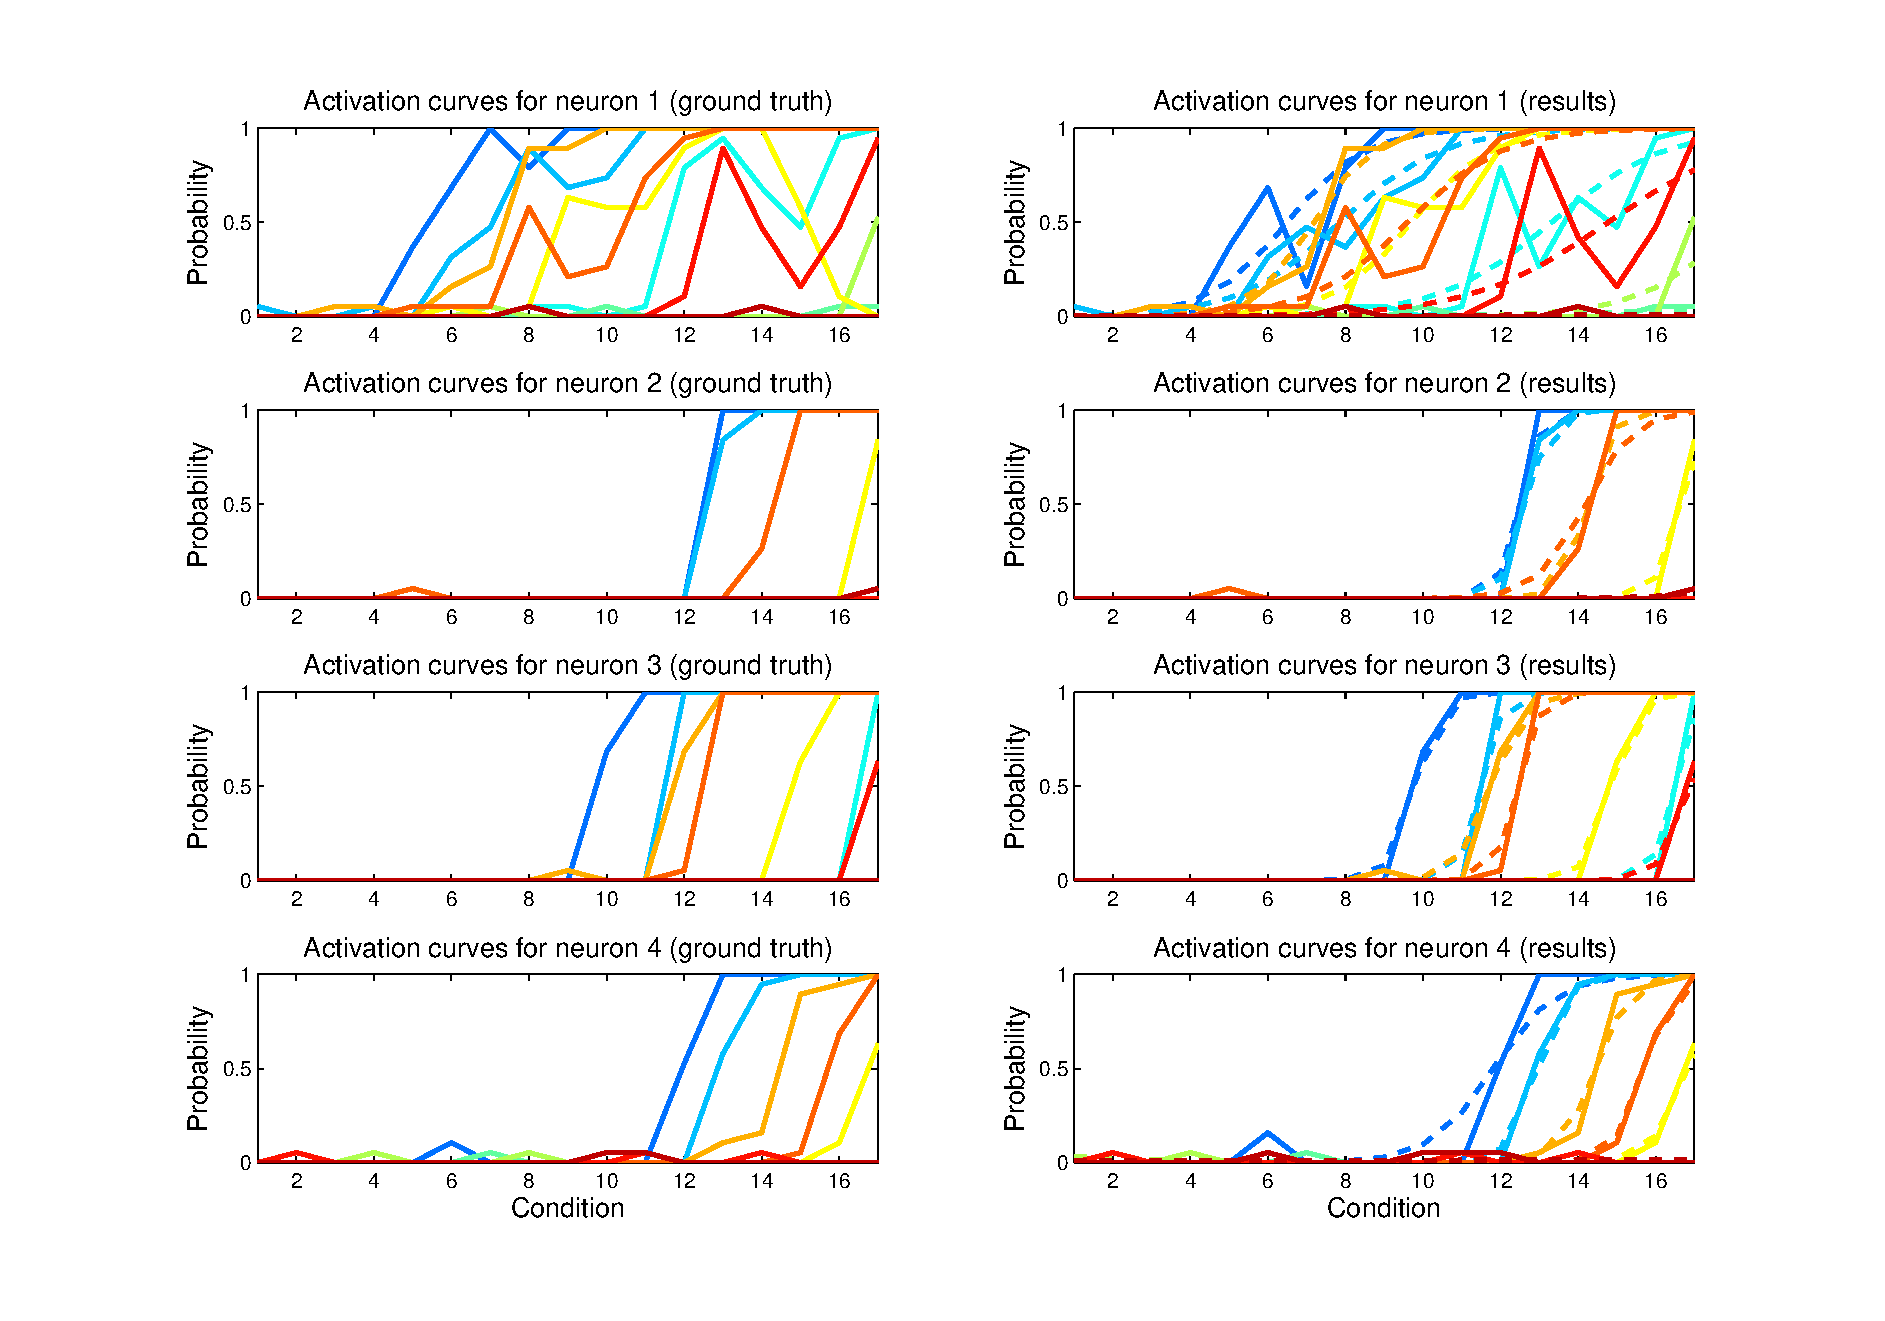
\includegraphics[width=1\textwidth]{Results10datasets.eps} 
                \caption{Activation curves, ground truth (left) and model results (right). Each trace corresponds to a dataset. In the  plots  to the right are also shown (dashed lines) the logistic regression fits}\end{figure}

\begin{table}[h!]
\begin{tabular}{|c|c|c|c|c|c|}
\hline
   &  Trials w. spikes & Failures in detection & Trials w. no spikes & False positives  & Total \\ \hline
   Neuron 1 & 4328 & 1019 (23.5\%) & 5940 & 490 (8.26\%) & 10268 \\ \hline
   Neuron 2 & 3515 & 689 (19.56\%) & 6236 & 519 (7.68\%)  & 10268\\ \hline
   Neuron 3 & 1498 & 0 & 8488 & 282 (3.22\%)& 10268  \\ \hline
   Neuron 4 & 2143 & 124 (5.79\%) & 7159 & 491 (11.89\%) & 10268  \\
  \hline
\end{tabular}
\caption{Overall results for all the analyzed neurons (all the 56 datasets)}
\end{table}


        \subsection{Misspecification due to axonal activation}
 It has been recently documented \cite{Lauren2014} that besides action potentials elicited by the targeted electrical stimulation of somas, there can be unwanted activation of axons. This activity can also be detected in electrode recordings, and although it is still not completely understood, it is known that begins to appear at a similar amplitude that of somatic spikes. However, unlike somatic spikes, the magnitude of this aggregated activation of axons increases with stimulus amplitude, and the activation curves of these axonal activities tend to be much sharper than of spikes. Because of this, templates are not available for this bundle activation and as a result it cannot be easily accounted for in the current framework. 
 \\ Axonal activation thus leads to model misspecification, and the question is to which extent our misspecified model can still be useful to detect spikes, in other words, will this phenomenon affect algorithm performance, and if it does, is it possible to inform a possible failure, in order to proceed with manual detection?\\
To address this questions we proceed via examples. In figure 4 is shown an example of successful detection (although it doesn't coincide with ground truth) regardless of the presence of axonal activation. This example serves to illustrate a way in which axonal activation interacts with the rest of the components of the model: here, spikes have a bigger magnitude than the corresponding template, and this is explained by the overlap in time of somatic and axonal spikes. Thus, we detect onset of axonal activation by increased residual variance $\sigma$ (in this case conditions 11 or 12). Also, once axonal activation becomes less variable in time, it is treated by the algorithm as being part of the artifact, which explains the difference in red and black traces at conditions 14 and 15. There are some cases, however, where the spike shapes change so much due to axonal activation that the templates are not good enough to explain the residuals and as a result spikes are failed to be detected. This is a rare situation, and again, it should be identified by an increased residual variance. An example of failure is shown in figure 5. There are conditions (e.g. 6,7) in which clusters naturally into three classes: no spiking, spiking and spiking plus axonal activation. At conditions 7 and 8 spikes are not detected, and only spike plus axonal activation trials are considered as true spikes (in fact, the same judgement was made by the human at condition 8). To understand how things can go wrong here it is important to look at the residuals: In some sense, it is also a meaningful interpretation to believe blue traces in condition 7 have no spikes, because if that was the case the spike template would fairly match the residuals. This example shows how spike sorting requires a level of expertise that is beyond what can be stated in the model. However, again in this case presence of axonal activation is indicated by increased residual variance, which can be informative for the experimenter. Other examples (not shown here) include similar situations, and an erroneous spike detection could be detected by a lack of fit between the activation curves and the underlying logistic model. Finally, another measure that can be informative comes from the regularization prior: basically, one can ask the question of how plausible is our artifact estimate given our prior artifact specification. If not, that could indicate that a artificial breakpoint should be added to the model in order to properly account for the changes in the artifact induced by the axonal activation. 
\\Summarizing, this modeling framework is not exempt of risks due to misspecification, but we can evaluate the goodness of fits by looking at different relevant aspects of the model: underlying spike probabilities, residual variances, and prior artifact specification. Taken together they should lead to relevant information about possible lack of fit, causes of this lack of fit (axonal activation) and ways in which this lack of fit could be driving the results wrong.
\pagebreak
\begin{figure}[h!]
          \centering
                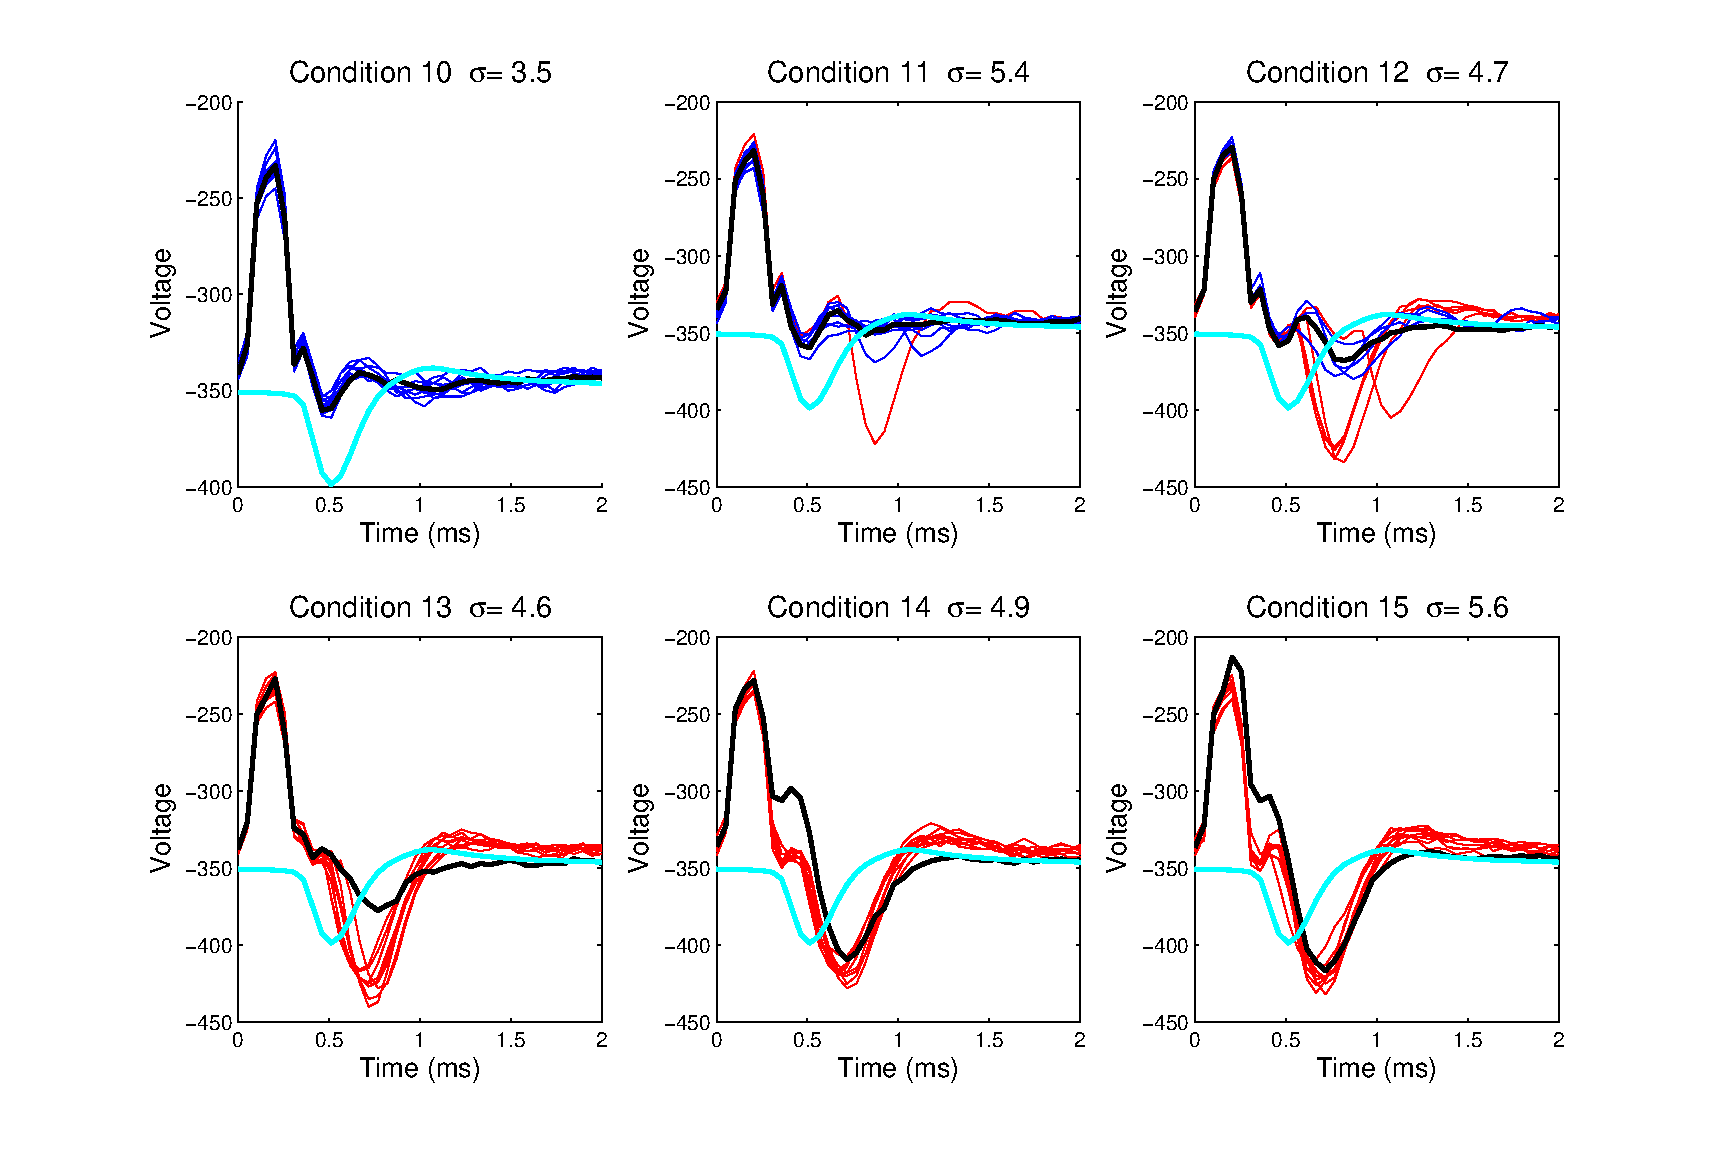
\includegraphics[height=4in]{TracesEl185pattern1494.eps} 
                \caption{An example of successful detection with axonal activation. Cyan trace: spike template, blue traces: trials with no spike, red traces: trials with spikes, black: artifact estimate}
\end{figure}


 \begin{figure}[h!]
        \centering
        \begin{subfigure}[b]{\textwidth}
                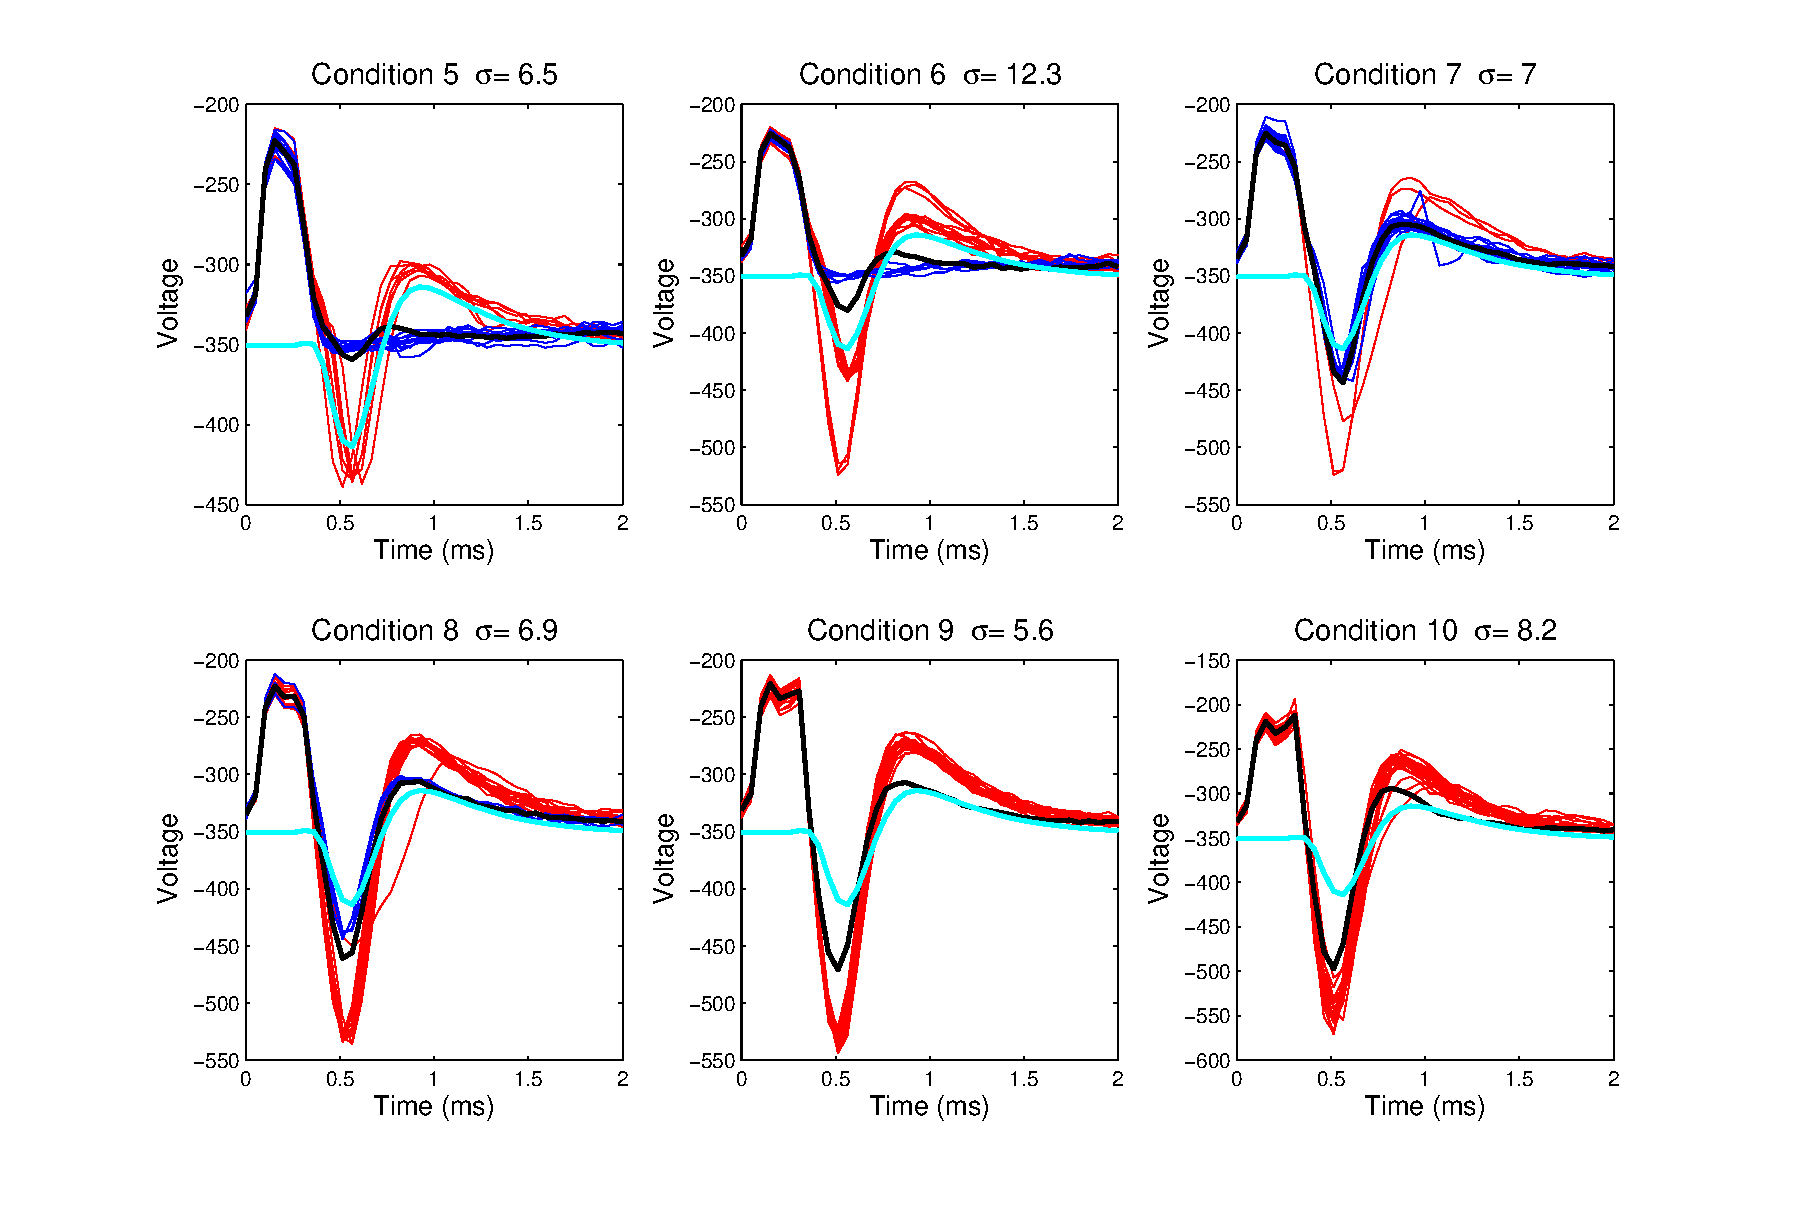
\includegraphics[height=4in]{TracesEl170pattern1443.eps}
   \caption{Traces}
                \label{fig:gull}
        \end{subfigure}% 
\centering

\begin{subfigure}[b]{\textwidth}
                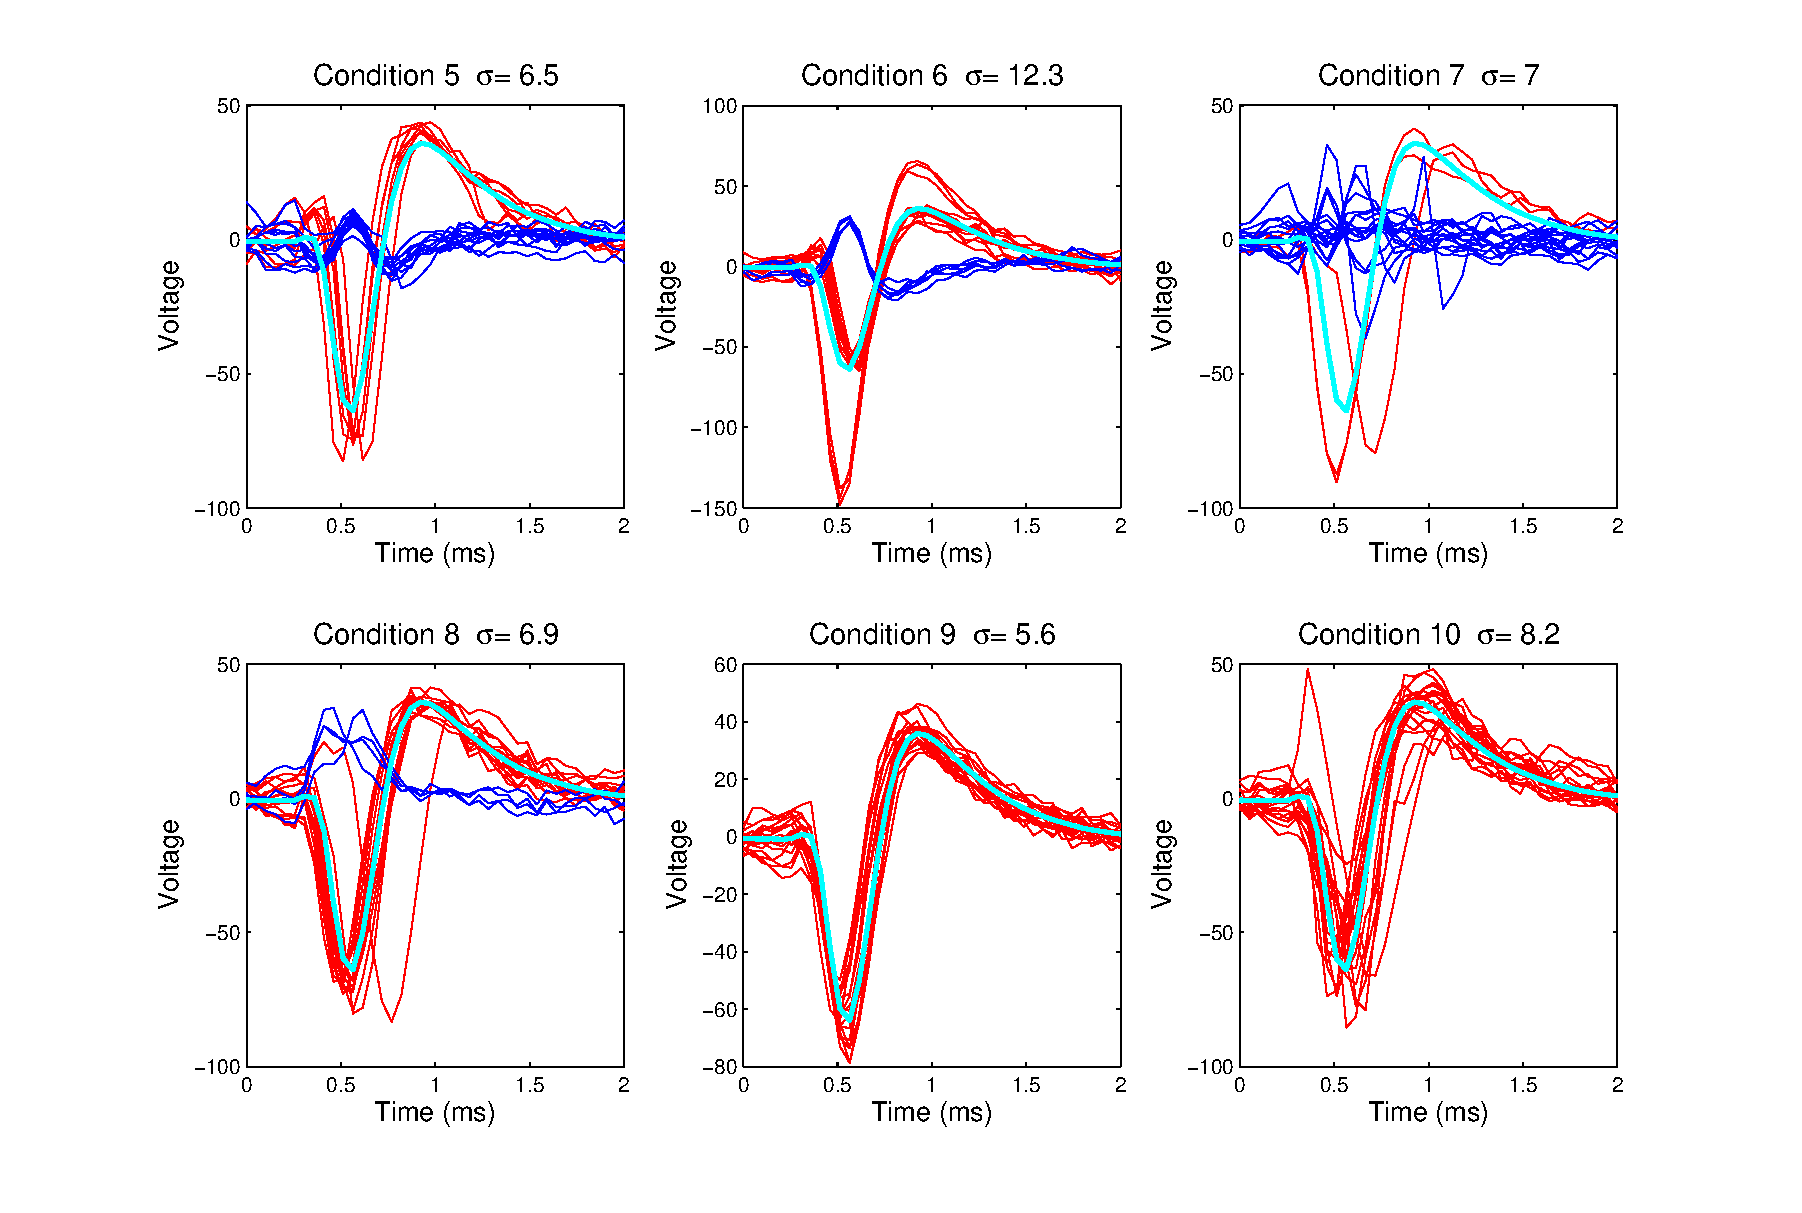
\includegraphics[height=4in]{ResidualsEl170pattern1443.eps}
                \label{fig:tiger}
                \caption{Artifact substracted residuals}
        \end{subfigure}
\caption{An example of failure in detection with axonal activation. Cyan trace: spike template, blue traces: trials with no spike, red traces: trials with spikes, black: artifact estimate}
\end{figure}
